\section{Rubin Observatory Commissioning}
\label{sec:commissioning}

\subsection{Commissioning Schedule}
\label{ssec:commissioning-schedule}

Following the October 2023 project schedule workshop, the Rubin Construction Project is re-optimizing the sequence of integration activities in light of recent subcomponent delays, in particular, (i) delay in shipment of the Camera and (ii) necessary repairs to the  summit dome crane.
If current estimates hold, it will be beneficial to re-implement on-sky data-taking with ComCam (previously removed from the schedule in order to install LSSTCam sooner).
The updated plan calls for on-sky data to be taken with ComCam for approximately two months, around July-August 2024 to support Telescope commissioning, primarily the Active Optics System. 
This is approximately four months earlier than could be done with LSSTCam. 

\begin{figure}[htb]
\centering
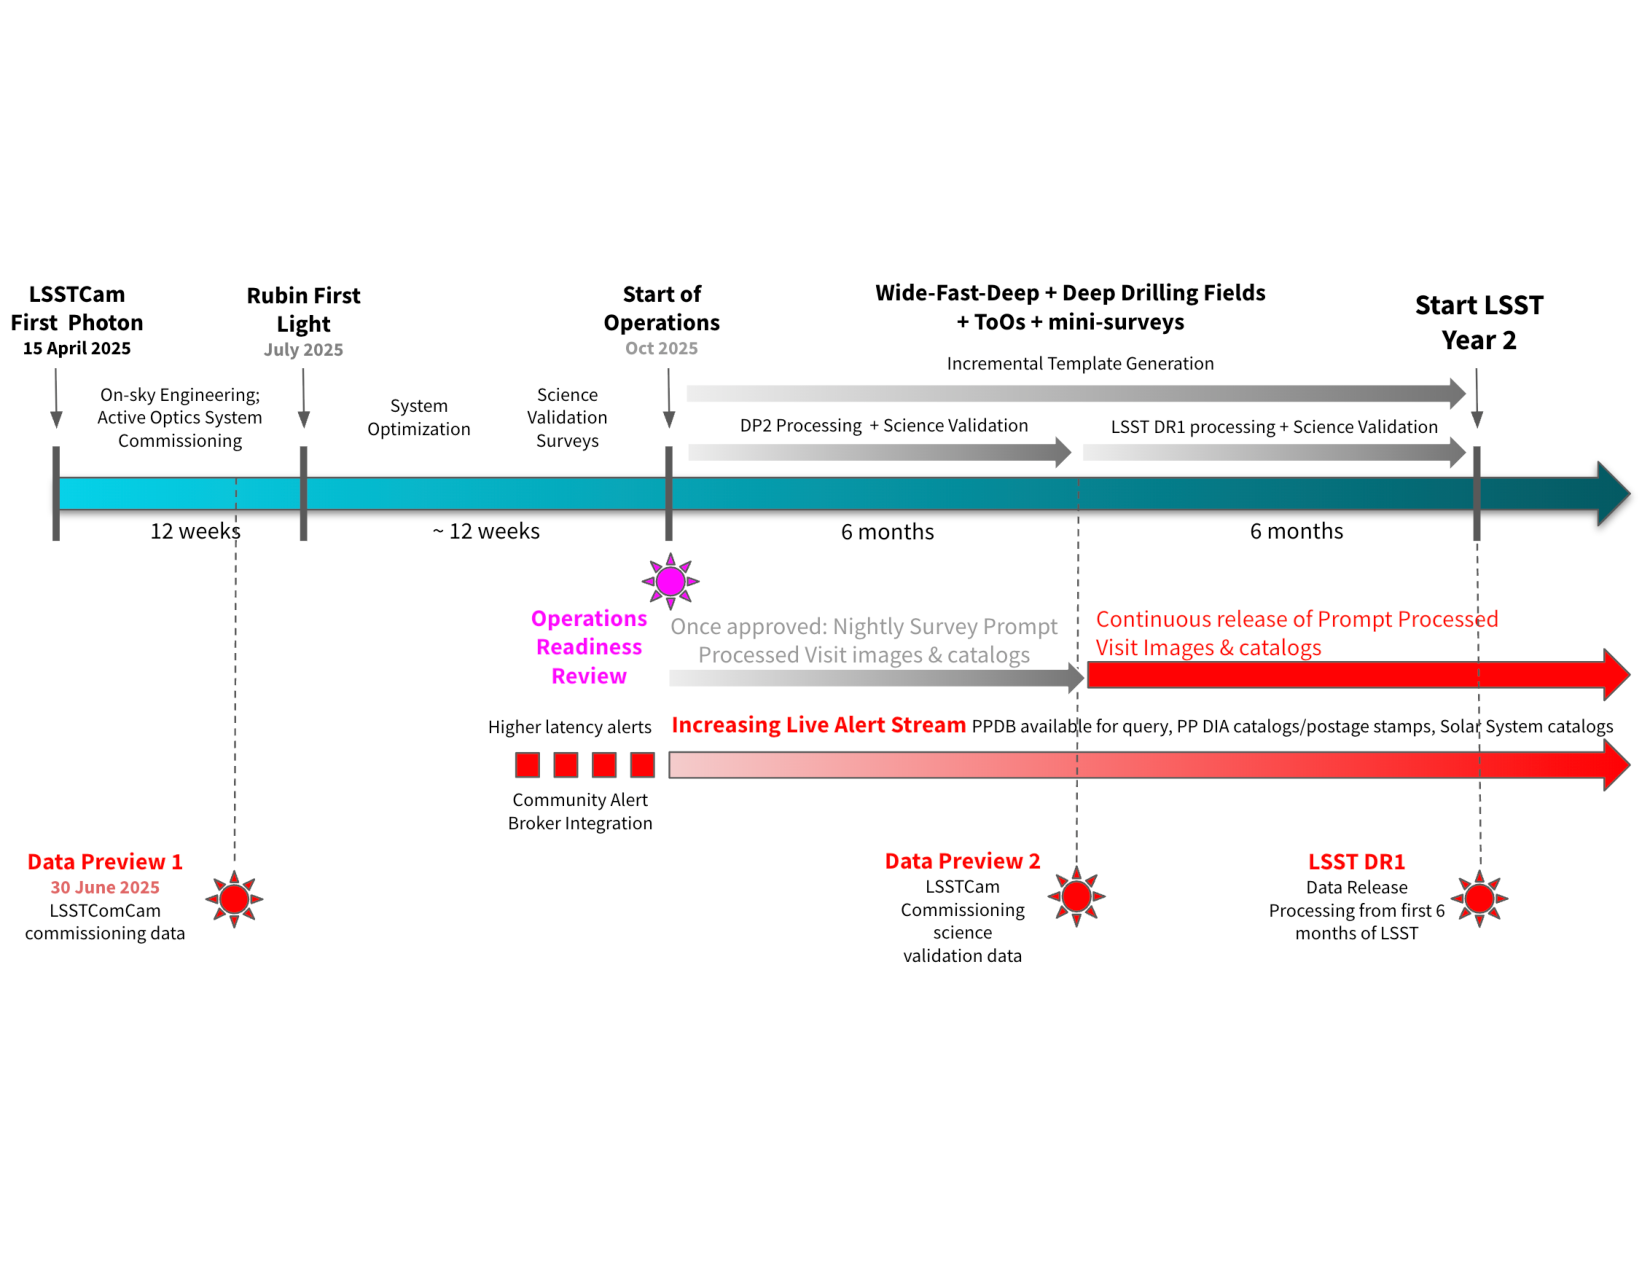
\includegraphics[width=0.98\linewidth]{figures/rubinobs_on-sky_commissioning_and_early_science.pdf}
\caption{Detailed schedule of commissioning  and early science activities relative to System First Light, as of October 2023.}
\label{fig:commissioning-es-schedule}
\vspace{0.1cm}
\end{figure}

Figure~\ref{fig:commissioning-es-schedule} shows the detailed schedule of commissioning and early science activities relative to System First Light, as of October 2023.
System First Light is currently expected in January 2025 (\S~\ref{sec:timeline}), about 7 weeks after LSSTCam First Photon.
The total amount of science validation time currently planned is about 8 weeks.  
LSST data taking is expected to start 4-10 months after System First Light depending on construction schedule uncertainty and Operations readiness to start the survey following the start of full Survey Operations.

The project schedule will continue to evolve as the remaining subcomponents are delivered. 
The final decision concerning ComCam on-sky data taking will be taken in February 2024.

\subsection{Commissioning Milestones}
\label{ssec:commissioning-milestones}

Commissioning work is being planned around three major milestones, \textit{ComCam First Photon}, \textit{LSSTCam First Photon} and \textit{System First Light}. 

\textbf{ComCam First Photon}: The first image of the night sky produced by photons passing through the Rubin optical system and detected by the Commissioning Camera (ComCam).

\textbf {LSSTCam First Photon}: The first image of the night sky produced by photons passing through the Rubin optical system and detected by the LSST Science Camera (LSSTCam).

\textbf {System First Light}: Defined as the point at which we can routinely acquire science-grade imaging across the LSSTCam full focal plane and have a well understood technical path towards meeting the Construction Completeness criteria   \citeds{sitcomtn-061}.
Also referred to as \textbf{First Light}. 

As the Project continues to optimize the sequence of integration activities and if it becomes no longer beneficial to go on-sky with ComCam, the ComCam First Photon milestone will be descoped. 
LSSTCam First Photon occurs following the successful completion of system integration. 
There are no quality criteria applied to achieving  neither the ComCam nor LSSTCam First Photon milestones. 
System First Light  marks the end of the  on-sky engineering phase and the start of the System Optimization and Science Validation phases of commissioning.
During the period between ComCam First Photon and System First Light will focus on fine tuning the system including optical alignment and improving the image quality, collecting calibration data, and carrying out \textit{First Look} science programs. 

For a detailed description of all the commissioning milestones and the most current dates, see \citeds{dmtn-232}.


\subsection{Commissioning Observations}
\label{ssec:commissioning-observations}

Figure~\ref{fig:commissioning} shows the high level plan for the Rubin commissioning observations. 
Commissioning data collection is planned to take place in phases.
The \textit{On-Sky Engineering} phase may be carried out with either ComCam and/or LSSTCam, depending on future re-optimization of the sequence of integration activities (\S~\ref{ssec:commissioning-schedule})
During the \textit{System Optimization} phase,  a set of observations designed to help optimize the system will be taken during the System Optimization phase before the Science Validation Surveys are carried out. 
The SV Surveys are designed to support scientific analyses that validate the system's performance, and allow Rubin to demonstrate operations readiness \citeds{SITCOMTN-005}.

\begin{figure}[htb]
\centering
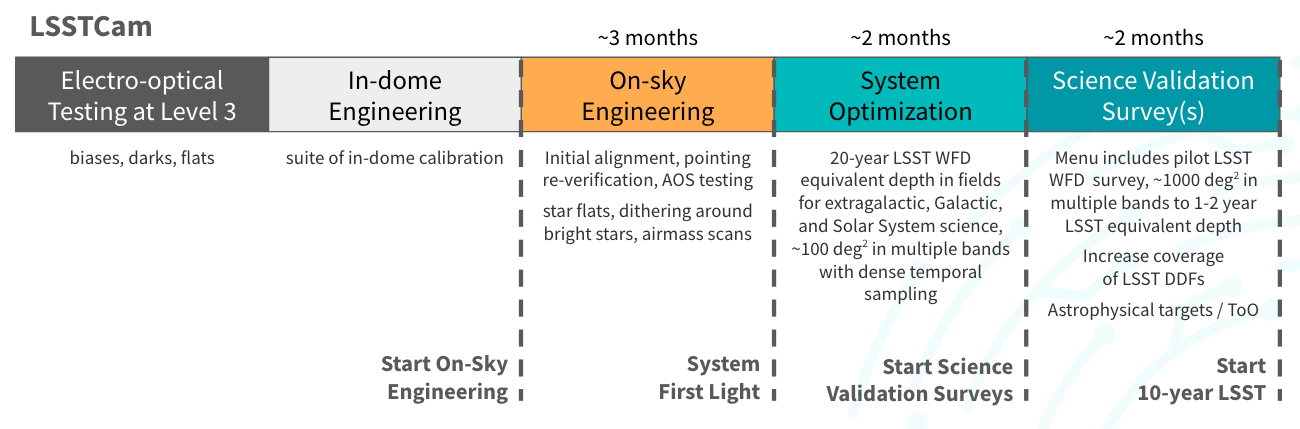
\includegraphics[width=0.95\linewidth]{figures/commissioning-plan}
\caption{Outline plan for the collection of commissioning data, as of October 2023.}
\label{fig:commissioning}
\end{figure}

Figure~\ref{fig:commissioning} also indicates a number of planned key components of the System Optimization and SV phases.
These include a LSST wide-fast-deep (WFD) 1-2 year equivalent depth ``pilot'' survey.
Field selection will be carried out by the Commissioning Team, taking into account a wide variety of constraints as well as a ``menu'' of science opportunities to which the LSST Science Community has contributed.
Details of the plans for commissioning observations will be made available as those plans converge, in this technote and other documents as cited.